\documentclass[11pt]{article}
\usepackage{icmlko}
\begin{document}

\title{축이 없는 행을 신호가 없다고 읽었다 --- 노트 360 다시 재기}
\author{월드모델 실험실}
\date{노트 377 · 2026년 8월 1일}
\maketitle

\begin{abstract}
노트 376이 좁은 퍼짐 대조를 만드는 법을 정했다 --- 무작위 부분집합이
아니라 \textbf{라벨 순 연속 창}이다. 그리고 자기 남은 것에 적었다:
\emph{노트 360이 팝업 주최자 주장을 ``무신호''라 부를 때는 이 대조가
없었다.} 그 대조를 돌렸다.

\textbf{대조는 애매했다.} 주장 57행의 유보 $\rho$ 는 $+0.1034$ 인데,
실측에서 같은 퍼짐의 연속 창 133개를 잘라 만든 띠가
$[+0.0721,\ +0.4594]$ 라 8번째 백분위로 \emph{안}이다. 그런데 어림수로
불린 14행을 빼면 4번째 백분위로 \emph{밖}이 된다. 어느 쪽이든 확실한
것은 하나다 --- 퍼짐이 좁아서 낮은 것은 \textbf{아니다}. 범위를 맞춰도
실측 중앙은 $+0.35$ 인데 주장은 $+0.11$ 이다.

\textbf{애매함을 가르다가 진짜 이유를 찾았다.} 어림수 주장 14행에 대한
모형의 예측이 \textbf{전부 같은 한 값}이었다. 세어 보니 주장 114행의 공유
축 덮음이 \textbf{12.3\%}(실측 89.3\%)이고, \textbf{87.7\%는 축이 하나도
없다.} 노트 360이 ``무신호''라고 쓴 것은 라벨에 대한 말이 아니라
\textbf{우리 설계행렬의 빈 칸}에 대한 말이었다. 그 행들은 시험받은 적이
없다.

빈 칸인 이유도 우연이 아니다. 팝업 자동 태거는 존재하고 932건을 예측하는데,
하네스가 쓰는 \emph{공유} 축 다섯의 재현 $\rho$ 가 $0.15\ldots0.41$ 이고
태거가 잘 맞히는 축들($0.51\ldots0.59$)은 하필 팝업 전용이라 안 쓰인다.
그래서 \texttt{min\_rho=9.9} 로 채움이 통째로 꺼져 있었다 --- 근거 있는
선택이지만 \emph{한 번도 다시 재지 않은} 선택이다.

\textbf{그래서 채워서 재봤다 --- 더 나빠진다.} 짝지은 부트스트랩 12회에서
팝업이 채움만 $-0.0367$ · 주장 넣고 안 채움 $-0.0694$ · 굿즈만 채움
$-0.0805$ · 다섯 다 채움 $\mathbf{-0.1411}$ 로 \textbf{채울수록 단조로
나빠지고 넷 다 12뽑기 중 두 번 이하로만 이긴다}. 빈 칸을 아는 것으로
바꾸면 되는 게 아니었다 --- 채울 수단이 그 다섯 축에 대해서는 잡음이다.
\texttt{min\_rho=9.9} 라는 한 줄이 처음으로 \emph{측정}으로 정당화됐다.

노트 360의 판정은 유지된다. 그러나 이유가 바뀌므로 이름도 바꾼다:
팝업 주장은 무신호형이 아니라 \textbf{빈칸형}이다 --- 신호가 없다고
쟀던 게 아니라 \emph{잴 열이 없었고, 채울 수단은 잡음}이다.
\end{abstract}

\section{왜 이것을 골랐나}

노트 376의 남은 것 표에서 값이 제일 큰 항목이었다. 팝업은 학습이 24행뿐인
--- 판에서 제일 얇은 --- 도메인인데 동시에 \textbf{배포 도메인}이라 노트
367 이후 판이 미결정일 때마다 결정을 내린다. 주장 행을 쓸 수 있으면 학습이
141행으로 여섯 배가 된다. 노트 360이 그 길을 ``무신호''로 닫았고, 노트
376이 그 판정에 대조가 없었다고 짚었다.

\begin{figure}[t]
\centering
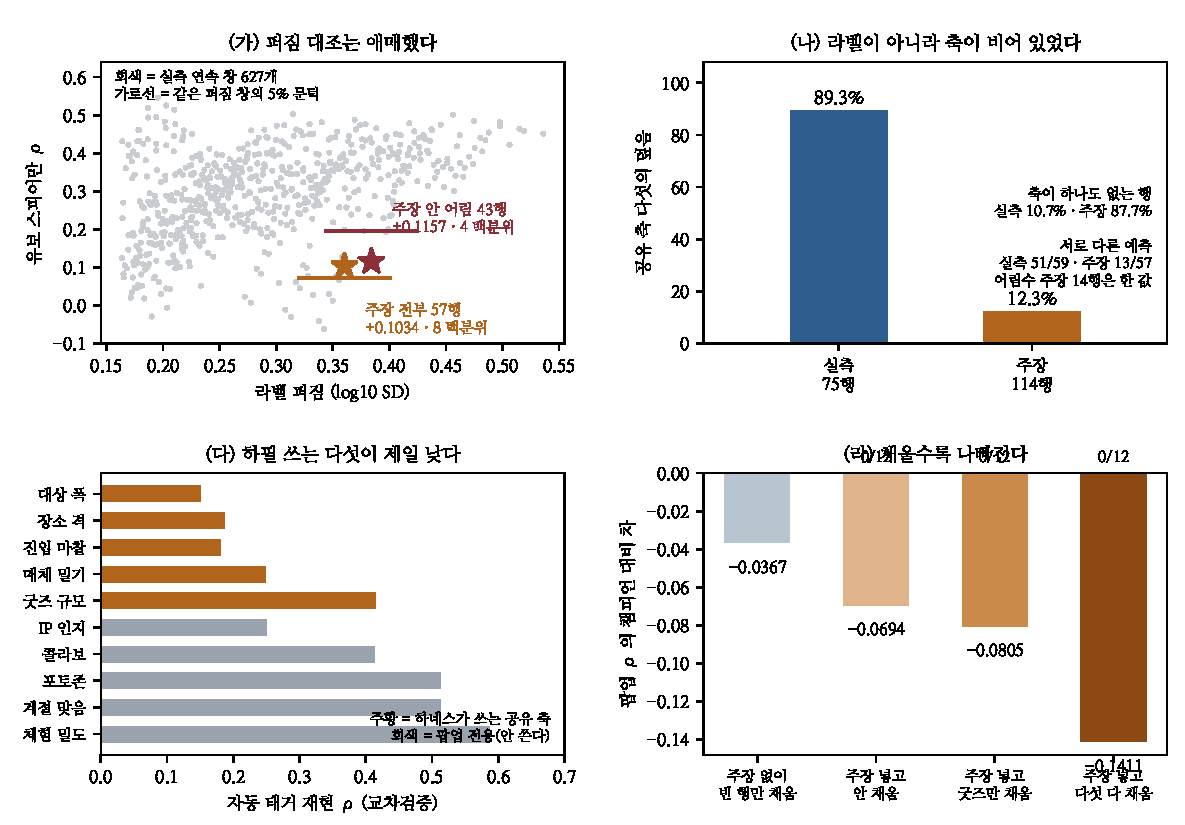
\includegraphics[width=\linewidth]{figs/fig377.pdf}
\caption{\textbf{(가)} 실측 59행에서 라벨 순 연속 창을 크기 25\,--\,57로
627개 잘라 (퍼짐, $\rho$) 를 찍었다. 주장은 자기 퍼짐에 맞는 창들의 5\%
문턱(가로선) 근처에 걸린다 --- 전부는 8백분위로 안, 어림수를 뺀 43행은
4백분위로 밖. \textbf{(나)} 그 애매함의 정체. 주장 행은 공유 축 덮음이
12.3\% 이고 87.7\%는 축이 하나도 없다 --- 모형이 잴 수가 없다.
\textbf{(다)} 왜 안 채웠나. 자동 태거는 팝업 전용 축(회색)은 $\rho\,0.5$
넘게 맞히는데 하네스가 쓰는 공유 축 다섯(주황)은 $0.15\ldots0.41$ 이다.}
\label{fig:main}
\end{figure}

\section{퍼짐 대조 --- 그리고 왜 창 하나를 고르지 않았나}

챔피언 F18@\texttt{idolwide\_full} 을 학습(2025년 전)에 한 번 적합시키고
팝업 유보를 계수 기준으로 갈랐다. \texttt{entry}\,·\,%
\texttt{participation} 이 실측, \texttt{organizer\_claim} 등이 주장이다.
\textbf{한 번의 적합 안에서 가른다}(노트 372 절차) --- 따로 적합시키면
도메인 칸의 부호가 열에 넷 뒤집힌다(노트 358).

주장의 라벨 퍼짐이 실측의 63\% 라, 낮은 $\rho$ 가 (i) 신호가 없어서인지
(ii) 범위가 좁아서인지 갈라야 한다. 실측 59행을 라벨 순으로 정렬하고 크기
$k=25\ldots57$ 의 연속 창을 \textbf{전부} 잘라 627개의
$(\mathrm{SD},\rho)$ 를 모은 뒤, 견줄 부분집합의 퍼짐 $\pm0.04$ 안에 드는
창으로 띠를 만들었다.

\textbf{처음 시도는 실패했고 그것이 갈래를 열었다.} 창 크기를 주장과 같은
57로 고정했더니 실측 59행 중 57행이라 창이 셋뿐이고 퍼짐이 0.506
까지밖에 안 좁아진다 --- 대조가 성립하지 않는다. 크기를 풀어야 퍼짐이
맞고, 크기를 풀면 $\rho$ 가 창 자리에 따라 $+0.01$ 에서 $+0.51$ 까지
흔들린다. \textbf{그래서 제일 잘 맞는 창 하나를 고르지 않고 띠 전체를
썼다.} 하나만 골랐다면 창 30행($+0.0125$)을 집어 ``주장이나 실측이나
똑같다''고 쓸 수도, 창 50행($+0.4020$)을 집어 ``주장은 무신호''라 쓸 수도
있었다. 노트 133이 첫 양수를 그대로 채택하지 말라 한 것의 대조판이다.

\begin{center}
\begin{tabular}{lrrrl}
\hline
부분집합 & 행 & 퍼짐 & $\rho$ & 실측 같은 퍼짐 띠 \\
\hline
주장 전부 & 57 & 0.360 & $+0.1034$ & $[+0.0721,+0.4594]$ · 8백분위 · \textbf{안} \\
주장 안 어림 & 43 & 0.384 & $+0.1157$ & $[+0.1948,+0.4590]$ · 4백분위 · \textbf{밖} \\
주장 어림 & 14 & 0.273 & 정의 안 됨 & 예측이 \textbf{상수} \\
\hline
\end{tabular}
\end{center}

판정이 부분집합에 따라 5\% 선을 넘나든다. \textbf{애매하다고 적고
넘어가지 않았다} --- 마지막 줄이 왜 ``정의 안 됨''인지를 봤다.

\section{예측이 상수였다 --- 진짜 이유}

어림수로 불린 주장 14행에서 모형의 예측이 전부 같은 한 값이라 스피어만이
계산되지 않는다. 서로 다른 예측의 수를 세면 실측 59행은 51개, 주장 안
어림 43행은 12개, 주장 어림 14행은 \textbf{1개}다.

설계행렬을 봤다.

\begin{center}
\begin{tabular}{lrrr}
\hline
 & 행 & 공유 축 덮음 & 축이 하나도 없는 행 \\
\hline
실측 & 75 & 89.3\% & 10.7\% \\
주장 & 114 & \textbf{12.3\%} & \textbf{87.7\%} \\
\hline
챔피언(실측만) & 89 & 83.1\% & 16.9\% \\
\hline
\end{tabular}
\end{center}

\textbf{주장 행의 열에는 값이 거의 없다.} 마스크가 0 이면 모형은 도메인
기본값을 낸다 --- 그래서 상수다. 노트 360이 ``무신호''라 쓴 것은
\emph{주최자 주장이라는 라벨에 정보가 없다}는 뜻으로 읽혔지만, 실제로
잰 것은 \emph{그 행들에 축이 안 채워져 있다}는 것이었다. 두 문장은 전혀
다르고, 뒤엣것은 우리가 고칠 수 있다.

\section{왜 비어 있었나 --- 근거는 있었다}

\texttt{popupset.build} 는 \texttt{mode} 가 \texttt{tag} 또는
\texttt{claim} 일 때 자동 태거로 빈 축을 채우되 재현 $\rho$ 가
\texttt{min\_rho} 미만인 축은 안 채운다. 그런데 \texttt{loop.py} 가
\texttt{min\_rho=9.9} 를 넘긴다 --- $\rho\le1$ 이므로 \textbf{아무것도 안
채운다}. 채움이 통째로 꺼져 있었다.

근거는 있다. 태거의 교차검증 재현 $\rho$ 를 축별로 보면 체험 밀도 0.587 ·
포토존 0.513 · 계절 맞음 0.512 로 꽤 높은데, 이 셋은 팝업 전용이라
하네스가 안 쓴다. 하네스가 쓰는 공유 축 다섯은 굿즈 규모 0.414 · 매체 밀기
0.249 · 장소 격 0.187 · 진입 마찰 0.181 · 대상 폭 0.151 로 \textbf{하필
제일 낮다}. 평균 0.346 은 그 셋이 끌어올린 값이다.

\textbf{근거 있는 선택이지만 다시 잰 적이 없는 선택이다.} 노트 360은 채움이
꺼진 자료로 주장 행을 시험하고 못 쓴다고 적었다.

\section{채워서 재기 --- 관문}

노트 367 규약으로 짝지은 부트스트랩 12회를 돌렸다. 모든 팔이 팝업 유보
65행 · 분모 2,981로 \textbf{채점 집합이 같다}(노트 371).

\begin{center}
\begin{tabular}{llrrl}
\hline
팔 & 팝업 학습 & 축 덮음 & 팝업 $\rho$ 차 & 판정 \\
\hline
A 챔피언 & 24 & 83.1\% & --- & --- \\
G 주장 없이 빈 행만 채움 & 24 & 100\% & $-0.0367$ (2/12) & 판이 안 넣으라 함 \\
C 주장 넣고 안 채움 & 141 & 38.8\% & $-0.0694$ (0/12) & 배포가 안 넣으라 함 \\
E 주장 넣고 굿즈만 채움 & 141 & 51.1\% & $-0.0805$ (0/12) & 배포가 안 넣으라 함 \\
D 주장 넣고 다섯 다 채움 & 141 & 100\% & $\mathbf{-0.1411}$ (0/12) & 배포가 안 넣으라 함 \\
\hline
\end{tabular}
\end{center}

판 차이는 넷 다 $-0.002 \ldots -0.003$ 로 짝 SD 안이라 미결정이고, 배포가
0/12 로 정한다. G만 부호가 2/12 라 판이 직접 안 넣으라 한다.

\textbf{세 갈래로 갈랐고 셋 다 같은 쪽을 가리킨다.}

\textbf{첫째, 채움 자체가 해롭다.} G는 주장 행을 하나도 안 넣고
챔피언의 빈 16.9\% 만 채운 팔인데 벌써 팝업이 $-0.0367$ 이다. 주장
문제와 무관하게 \textbf{태거의 공유 축 채움이 잡음}이라는 뜻이고, 이것이
\texttt{min\_rho=9.9} 의 첫 실측 근거다.

\textbf{둘째, 채움의 양에 단조다.} 주장 141행을 고정하고 채움만 늘리면
$-0.0694 \to -0.0805 \to -0.1411$ 이다. 굿즈 규모($\rho\,0.414$) 하나만
채우는 것도 이미 손해고, 낮은 넷($0.151\ldots0.249$)을 더 얹으면 손해가
두 배가 된다.

\textbf{셋째, 둘이 겹친다.} 채움만 $-0.0367$, 주장만 $-0.0694$, 둘 다
$-0.1411$ --- 더한 값 $-0.1061$ 보다 더 나쁘다. 축 없는 행 117개를 넣는
것과 그 행들을 잡음으로 채우는 것은 서로를 악화시킨다.

\textbf{그리고 수준 때문이 아니다.} 네 팔 모두 계수 기준 안에서 학습
라벨의 중앙을 뺐다(노트 360의 \texttt{norm}). 2.58배 부풀림은 이미
제거된 상태이고 그래도 안 된다.

\section{규약에서 빠진 조항 하나}

이번에 팔 하나(\texttt{wide\_pop="train"})가 등급 A·B 로 떨어지면서 팝업
유보가 65행에서 59행으로 바뀌었다. 그 팔은 판 $-0.0035$ · 4/12 로
``미결정 $\to$ 배포가 정한다''가 되고 팝업이 $+0.0243$ · 9/12 로 \emph{넣으라}
한다 --- 그런데 그 $+0.0243$ 은 \textbf{다른 59행에서 잰 수}라 챔피언의
65행과 견줄 수 없다.

\textbf{노트 367 규약에 ``두 팔의 채점 집합이 같아야 한다''가 안 적혀
있다.} 적어 둔다: 채점 집합이 달라지는 팔은 미결정이 아니라
\textbf{잴 수 없음}이고, 배포가 정할 자격도 없다.

\section{덤 --- \texttt{COUNT\_OK} 한 줄이 어떤 축보다 값이 크다}

같은 116행에서 채점 방식만 바꿔 봤다: 실측만 $+0.4285$ · 주장만
$+0.1034$ · 따로 재고 가중평균 $+0.2688$ · 합쳐서 $+0.2635$. 그런데
\textbf{``어느 자로 쟀나''라는 표시자 하나가 라벨과 $+0.4416$} 으로
챔피언의 합친 점수를 이긴다. 주장 라벨은 중앙이 실측의 2.58배이고(단측
MWU $p=1.1\times10^{-6}$) 어림 천 단위가 12.3\% 대 3.4\% 라 --- 세어서
나온 수가 아니라 불러서 나온 수다.

이것을 축으로 넣으면 안 된다. 표시자가 재는 것은 세상이 아니라 \emph{우리가
어떻게 쟀나}다(노트 326의 풀 그림자 · 노트 354의 배치 표시자). 대신 이것은
\texttt{popupset.build} 의 \texttt{counting in COUNT\_OK} 한 줄이 왜 값이
큰지를 말한다 --- 떼면 팝업이 $+0.4285 \to +0.2635$ 로 내려간다. 스무 노트
넘게 아무도 안 들여다본 줄이 판의 어떤 축보다 값이 크다.

\section{남은 것}

\begin{center}
\begin{tabular}{lll}
\hline
항목 & 왜 값이 큰가 & 어떻게 \\
\hline
공유 축용 태거 & 태거가 쓰는 다섯을 못 맞힌다 & 전용 축 셋($\rho\,0.5{+}$)을 공유로 올릴 수 있나 \\
팝업 실측 41행 & 학습 24는 판에서 제일 얇다 & 수집; 노트 359의 50\,--\,65 문턱 \\
균일 펀딩 2,500 & 지금 표본은 상위 19\% & 진행 중 \\
만화 바닥 아래 & 만화도 632에서 잘렸다 & 노트 376 절차 \\
\hline
\end{tabular}
\end{center}

\end{document}
